\documentclass[11pt]{article}
\usepackage[paperwidth=8.5in,paperheight=11in,textwidth=5.6in,top=0.9in,bottom=0.9in]{geometry}
\usepackage[T1]{fontenc}
\usepackage{lmodern,microtype,graphicx,booktabs,xcolor,enumitem,titlesec,float,amsmath}
\usepackage[most]{tcolorbox}
\usepackage[colorlinks,urlcolor=accent,linkcolor=accent]{hyperref}
\renewcommand{\familydefault}{\sfdefault}
\definecolor{accent}{HTML}{2A78D6}
\definecolor{ink}{HTML}{0B0B0B}
\definecolor{muted}{HTML}{52514E}
\definecolor{wash}{HTML}{F3F2EE}
\setlength{\parindent}{0pt}
\setlength{\parskip}{0.6em}
\setlist{nosep,leftmargin=1.2em}
\titleformat{\section}{\Large\bfseries\color{ink}}{}{0pt}{}
\titlespacing*{\section}{0pt}{1.4em}{0.3em}
\newcommand{\f}[1]{\texttt{#1}}
\newtcolorbox{quoteit}{enhanced,breakable,colback=white,colframe=white,borderline west={3pt}{0pt}{accent},
  left=10pt,right=4pt,top=2pt,bottom=2pt,fontupper=\itshape\color{muted}}
\newtcolorbox{panel}[1][]{enhanced,colback=wash,colframe=wash,arc=4pt,left=10pt,right=10pt,#1}
\newcommand{\stat}[2]{\begin{tabular}[t]{@{}c@{}}{\huge\bfseries\color{accent}#1}\\[2pt]{\small\color{muted}#2}\end{tabular}}
\newcommand{\who}[1]{\textbf{\color{accent}#1}}

% numbers from session.py (copy writing figures/timeline-optimization.png), at the time of writing
\newcommand{\wall}{162}\newcommand{\human}{5}\newcommand{\agent}{32}\newcommand{\usd}{5.58}

\begin{document}

{\small\color{muted}LAB NOTEBOOK \textbullet{} 2026-10-22 \textbullet{} 7 min read}\\[4pt]
{\fontsize{26}{30}\selectfont\bfseries\color{ink} Evolving a Float Kernel,\\ Then Checking It}\\[6pt]
{\large\color{muted} AlphaEvolve wrote 19 versions of a WENO5 kernel in float. Three beat the seed.
Verification showed why it helps, and found the event where no float kernel can help.}

\vspace{0.8em}
\begin{panel}
\centering
\stat{1.31$\times$}{lower error, scored window} \hfill \stat{2.73$\times$}{before $t=1.45$} \hfill
\stat{19/19}{checks pass} \hfill \stat{\$\usd}{in agent tokens}
\end{panel}

\section{The ask}

The last session (\f{report.tex}) ended with the optimize stage planned, calibrated and
red-teamed, and blocked on Google Cloud credentials. The scientist came back with:

\begin{quoteit}
Let continue the experiment I have GCP credentials.
\end{quoteit}

They also pasted the notebook settings they use elsewhere: project, engine, model, job size.

\section{Getting to launch}

The credentials weren't where the container looks. The agent checked \f{\textasciitilde/.config/gcloud}
(no ADC file, no host gcloud) before trying anything.

\who{``How should I login?''} Through the container itself, so the credentials land in the mounted
folder. \who{``Write that code to file so I can run.''} A three-line script went to \f{/tmp},
outside the repo. One login later the container had a token.

Three small mismatches followed, each fixed from the tool's own source, not guessed:
\f{ae} wants the numeric project number, not the name; it rejects the notebook's model preset
\f{GEMINI\_V3P0\_MIXTURE}, which in \f{ae} is just \f{gemini-3-flash-preview} at weight 1; and the
launch script crashed because \f{experiment start} does not print JSON.

\who{``Make the changes you need, and be careful with credentials.''} The agent fixed the script,
then searched the repo and logs for tokens, refresh tokens and keys (none), and confirmed
\f{results/ae/} is gitignored and the ADC file is mode 600.

\section{The run that scored nothing}

The first experiment, \f{exp-free-hyena}, finished in six minutes: 9 candidates, 9 nulls,
``invalid score''. Bad candidates, or a bad evaluator? The agent pulled one and scored it
by hand: 9.20, valid.

The bug was ours. \f{ae} copies \f{evaluator.py} into a fresh temporary folder and runs it there,
so the output path the evaluator derived from its own location pointed into that folder, whose
\f{results/} did not exist. The app creates only the last folder, and crashed. The red team had
run the evaluator in place, never the way \f{ae} runs it. One line in \f{evolve.py} (create the
parent first) fixed it for every future experiment, and the rerun scored 9 of 10.

\section{What evolution found}

\begin{figure}[H]
\centering
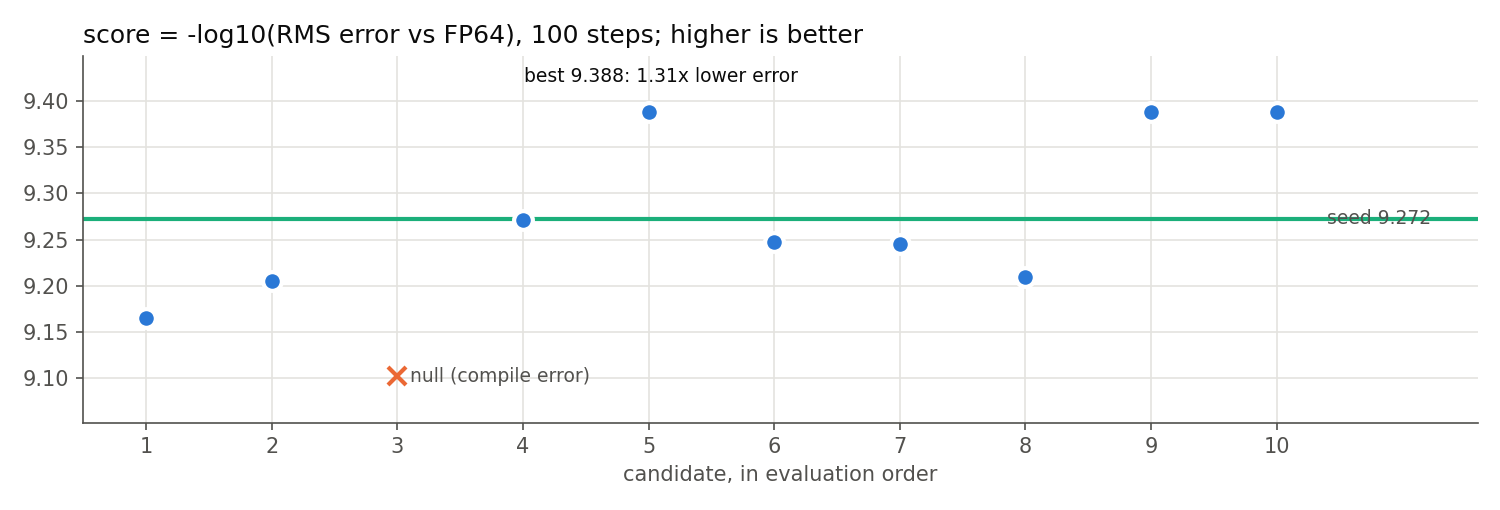
\includegraphics[width=\linewidth]{figures/verify_scores.png}
\caption{The second run, \f{exp-ginger-chimpanzee}: 10 candidates from Gemini 3 Flash, each built,
audited (no FP64 in the block, nothing changed outside it) and run in the container.}
\end{figure}

Three candidates tied near 9.388. They share one idea. The seed computes a WENO5 face value
as a weighted sum of three stencils, each of size $|\phi|$, whose large parts cancel:
\[
  f = a_1 f_1 + a_2 f_2 + a_3 f_3 .
\]
The candidates eliminate $a_2 = 1 - a_1 - a_3$ and write it as the centre value plus a small
correction built from neighbour differences $v_k = s_k - s_{k+1}$:
\[
  f = s_3 + \tfrac16\bigl(2a_1(v_1 - 2v_2 + v_3) + a_3(v_2 - 2v_3 + v_4) - v_2 - 2v_3\bigr).
\]
In a smooth field the differences are $O(\Delta x)$, so float rounds the small part, not the big
one. A textbook trick, found unprompted. Running all three to $t=2$ picked
\f{humongous-macaw}: tied at 100 steps, best over the full run.

\section{Verification}

\begin{center}
\begin{tabular}{@{}lrrr@{}}
\toprule
run & seed error & candidate & gain \\
\midrule
eval, $128^2$, 100 steps          & $5.34\times10^{-10}$ & $4.09\times10^{-10}$ & 1.31$\times$ \\
$256^2$, 200 steps                & $5.54\times10^{-10}$ & $4.36\times10^{-10}$ & 1.27$\times$ \\
to $t=2$, before the jump         & $9.12\times10^{-9}$  & $3.34\times10^{-9}$  & 2.73$\times$ \\
to $t=2$, after both jumps        & $4.87\times10^{-7}$  & $5.27\times10^{-7}$  & 0.92$\times$ \\
\bottomrule
\end{tabular}
\end{center}

All 19 checks pass. The field is bit-identical on 1, 2 and 4 ranks. Area and mass at $t=2$ stay
at fp32 level ($2\times10^{-6}$ off FP64; bf16 is $3\times10^{-3}$). And sympy confirms the
candidate's face value equals the seed's in exact arithmetic: the same scheme, rounded better.

\begin{figure}[H]
\centering
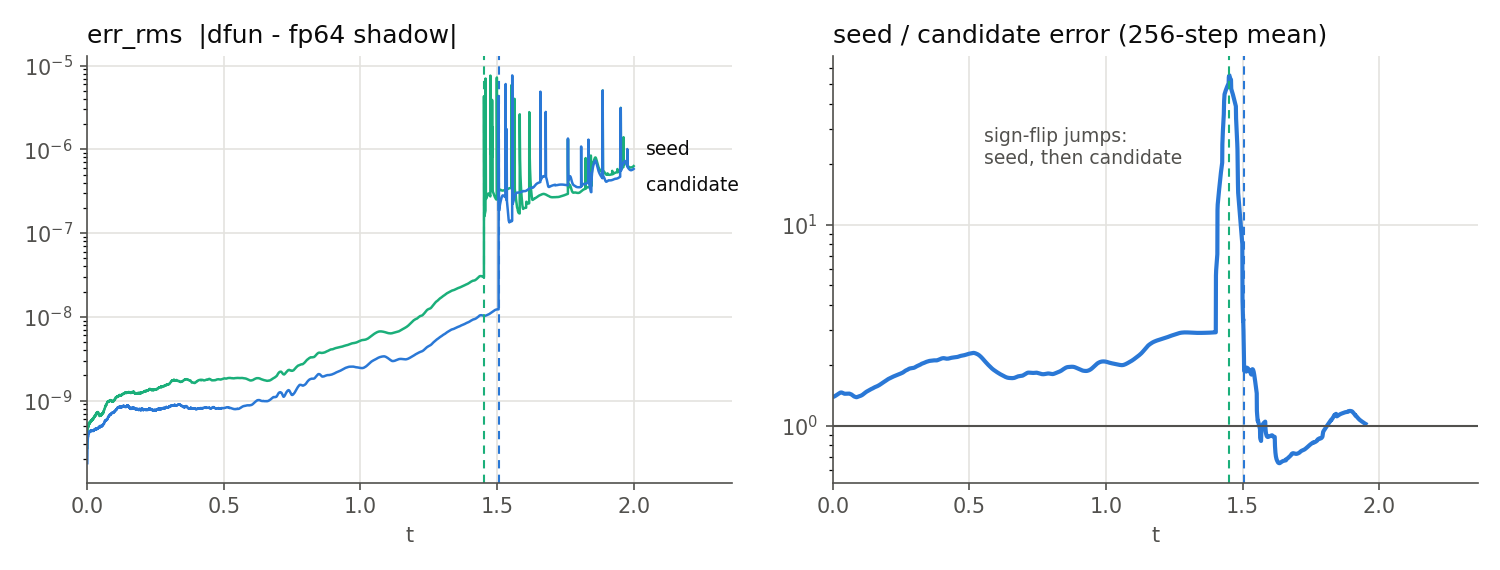
\includegraphics[width=\linewidth]{figures/verify_errors.png}
\caption{Error vs the FP64 shadow over the full run. The candidate stays 2--3$\times$ below the
seed until a jump at $t\approx1.45$ (seed) or $1.51$ (candidate); after it the two are alike.}
\end{figure}

\textbf{The jump.} In one step, the seed's largest error goes from $1.7\times10^{-7}$ to
$5.5\times10^{-4}$. Rerunning to the step before and after found one cell crossing zero:
$\phi=+1.18\times10^{-8}$ in FP64, $-3.25\times10^{-9}$ in float. The FP64 redistance tests for
interface cells by sign (\f{redistance.cpp:70}), takes the other branch, and the neighbour moves
by $5.5\times10^{-4}$: a 37\,000$\times$ amplification. Every low-precision run hits such
switches; better rounding only delays the first one by 275 steps. After that, sign flips decide
the error, not the kernel.

\begin{figure}[H]
\centering
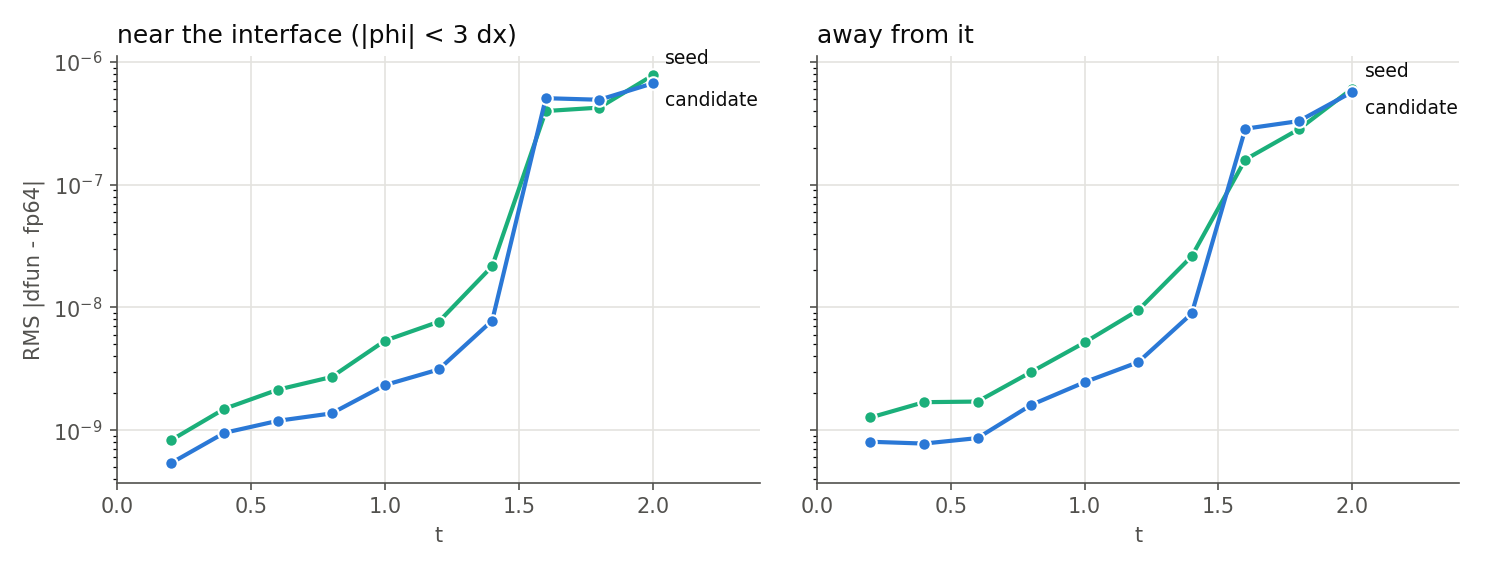
\includegraphics[width=\linewidth]{figures/verify_band.png}
\caption{The gain is the same near the interface and away from it, until the jump.}
\end{figure}

\textbf{Verdict (the scientist decides).} Merge: same scheme, more accurate while the flow is
smooth, no worse at $t=2$ overall. A further optimize run should score a window or a quantity the
sign switch cannot decide: $t<1.4$, $2\times$ resolution, or area and mass.

\section{How it went}

\begin{figure}[H]
\centering
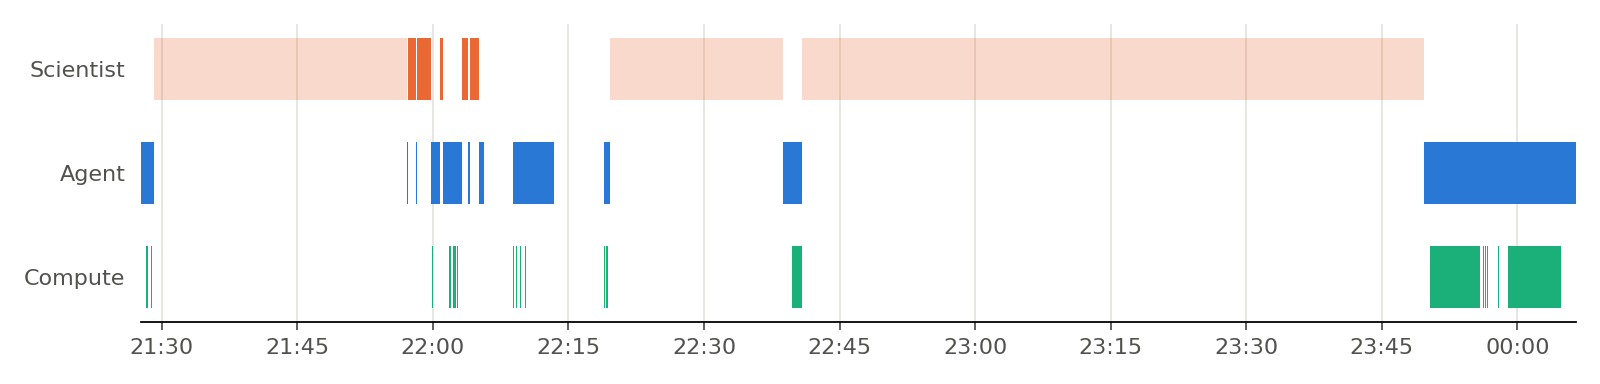
\includegraphics[width=\linewidth]{figures/timeline-optimization.png}
\caption{Pale orange: the scientist was away, mostly while AlphaEvolve ran on Google Cloud
(not on the compute lane, which counts local container runs only).}
\end{figure}

Nine messages, 120 words from the scientist. The longest one was \emph{``lets run verification
on these results and prepare a comprehensive report''}; the agent took that as approval of
Gate~2 and the verify plan, chose the defaults, and recorded each as its own choice in the plans.

\section{What it cost}

\begin{center}
\begin{tabular}{@{}lrrr@{}}
\toprule
Claude Opus 5.5, 108 calls & tokens & \$/M & \$ \\
\midrule
fresh input        & 218         & 4.00  & 0.00 \\
cache writes       & 519\,745    & 5.00  & 2.60 \\
cache reads        & 8\,416\,338 & 0.20  & 1.68 \\
output             & 64\,619     & 20.00 & 1.29 \\
\midrule
\textbf{total}     &             &       & \textbf{\usd} \\
\bottomrule
\end{tabular}
\end{center}

AlphaEvolve's side, 19 candidates over both runs: 58\,845 input and 612\,697 output tokens of
Gemini 3 Flash, billed to the GCP project (not priced here). Local compute: 16 minutes of container
runs, all of verification included.

\section{Human time vs.\ time saved}

\begin{panel}
\begin{tabular}{@{}p{4.3in}r@{}}
\multicolumn{2}{@{}l}{\textbf{Doing it by hand} \color{muted}(our estimate, for an expert new to \f{ae})}\\[2pt]
credentials, project number, model names, launch                  & 1 h \\
debug 9 nulls to the evaluator's working directory                & 1 h \\
re-score and full-run the top candidates, pick one                & 1 h \\
verification script, runs, the sign-flip hunt                     & 3 h \\
write this up with figures and costs                              & 2 h \\
\midrule
\textbf{total}                                                    & \textbf{$\approx$ 8 h} \\[4pt]
\textbf{With the agent:} scientist's attention                    & \textbf{\human{} min} \\
\end{tabular}
\end{panel}

The agent worked \agent{} of the \wall{} minutes; most of the rest was waiting on Google Cloud.

\section{What we'd change}

\begin{itemize}
  \item \textbf{Red-team the way \f{ae} runs:} copy \f{evaluator.py} to a temporary folder first.
    It would have saved a whole run.
  \item \textbf{Score past the easy window:} 100 steps hid the jump; 2.73$\times$ early, 1.17$\times$ overall.
  \item \textbf{Map notebook settings to \f{ae}:} presets like \f{GEMINI\_V3P0\_MIXTURE} and
    project names need translating; the stage could do it.
  \item \textbf{Still a papercut:} the app should create its output folder's parents.
\end{itemize}

{\sloppy\small\color{muted}Numbers: \f{3-verify/results/verify/summary.md}, \f{3-verify/analysis.md},
\f{2-optimize/results/scores.csv}; cost and timeline from \f{session.py} on this session's
transcript. Plans and patches are under \f{experiments/2026-10-20/}.\par}

\end{document}
